%----------------------------------------------------------------------------------------
% PACKAGES AND OTHER DOCUMENT CONFIGURATIONS
%----------------------------------------------------------------------------------------

% !TEX encoding = UTF-8
% !TEX TS-program = pdflatex
% !TEX root = rel_datamining.tex
% !TEX spellcheck = it-IT

\documentclass[a4paper, 11pt]{article} % Font size (can be 10pt, 11pt or 12pt) and paper size (remove a4paper for US letter paper)
\usepackage[italian]{babel}      							% Lingua italiana
\usepackage[margin=.9in]{geometry}             % Imposta i margini del documento

\usepackage[T1]{fontenc} % Required for accented characters
\usepackage[mathletters]{ucs}    % Caratteri matematici come UTF8
\usepackage[utf8,utf8x]{inputenc}      % Ancora utf8

\usepackage{eurosym}                %simbolo dell'euro
\usepackage{listings}
\usepackage[usenames,dvipsnames,svgnames,table]{xcolor}

%% !TEX encoding = UTF-8
% !TEX TS-program = pdflatex
% !TEX root = rel_datamining.tex
% !TEX spellcheck = it-IT

% Imposta lo spazio nella list of listing in modo simile alla list of figures/tables
%\makeatletter
%\let\my@chapter\@chapter
%\renewcommand*{\@chapter}{%
%  \addtocontents{lol}{\protect\addvspace{10pt}}%
%  \my@chapter}
%\makeatother


\definecolor{codegreen}{rgb}{0,0.6,0}
\definecolor{codegray}{rgb}{0.5,0.5,0.5}
\definecolor{backcolor}{rgb}{0.98,0.98,0.98}

\renewcommand{\lstlistingname}{Codice}% Listing -> codice
\renewcommand{\lstlistlistingname}{Elenco dei frammenti di codice}% List of Listings -> Frammenti di codice

\lstdefinestyle{mystyle}{
    backgroundcolor=\color{backcolor},   
    commentstyle=\color{Peach}\ttfamily,
    keywordstyle=\color{RoyalBlue},
    numberstyle=\tiny\color{codegray},
    stringstyle=\color{SeaGreen}\ttfamily,
    basicstyle=\footnotesize\ttfamily,
    breakatwhitespace=false,         
    breaklines=true,                 
    captionpos=b,                    
    keepspaces=true,                 
    numbers=left,                    
    numbersep=5pt,                  
    showspaces=false,                
    showstringspaces=false,
    showtabs=false,                  
    tabsize=2,
    frame=trbl, % draw a frame at the top, right, left and bottom of the listing
	frameround=ftff, % angolo in basso a destro curvo
	framesep=4pt, % quarter circle size of the round corners,
	inputencoding=utf8,
    extendedchars=true,
    literate={á}{{\'a}}1 {à}{{\`a}}1 {é}{{\'e}}1 {è}{{\`e}}1 {ù}{{\`u}}1 {ò}{{\`o}}1,
    belowskip=1em,
    aboveskip=1em,
}

 
\lstset{style=mystyle}

\lstdefinelanguage{JavaScript}
{
  % list of keywords
  morekeywords={ true, false, catch, function, break,	new, class, extends, var, require, switch, return, import, if, while, for, this, View, Text, StyleSheet},
  sensitive=false, % keywords are not case-sensitive
  morecomment=[l]{//}, % l is for line comment
  morecomment=[s]{/*}{*/}, % s is for start and end delimiter
  morestring=[b]' % defines that strings are enclosed in double quotes
}

\lstdefinelanguage{JSON}
{
  % list of keywords
  morekeywords={string, boolean, int, Array, Node, Asset, AssetDetail, Filter, FilterItem},
  sensitive=false, % keywords are not case-sensitive
  morecomment=[l]{//}, % l is for line comment
  morecomment=[s]{/*}{*/}, % s is for start and end delimiter
  morestring=[b]" % defines that strings are enclosed in double quotes
}

\lstdefinelanguage{URM}
{
	% list of keywords
	morekeywords={ S, J, T, Z, I},
	sensitive=false, % keywords are not case-sensitive
	morecomment=[l]{//}, % l is for line comment
	morecomment=[s]{/*}{*/}, % s is for start and end delimiter
	morestring=[b]' % defines that strings are enclosed in double quotes
}

%\tightlist per compatibilità con pandoc
\providecommand{\tightlist}{%
  \setlength{\itemsep}{0pt}\setlength{\parskip}{0pt}}


\usepackage[labelfont=bf]{caption}

\usepackage[protrusion=true,expansion=true]{microtype} % Better typography
\usepackage{graphicx} % Required for including pictures
\usepackage{wrapfig} % Allows in-line images


\usepackage{subfig}
\usepackage{hyperref}
\usepackage{mathpazo} % Use the Palatino font

\linespread{1.05} % Change line spacing here, Palatino benefits from a slight increase by default
\usepackage{placeins}
\usepackage{sourcecodepro}
\usepackage{hyperref}                   % collegamenti ipertestuali

\usepackage[colorinlistoftodos,prependcaption]{todonotes} %todo

\usepackage{amsmath}
\usepackage{subfig}
\usepackage{mathtools}
 \usepackage{multirow}
\usepackage{float}
\usepackage{algorithm}
\usepackage{algpseudocode} % https://en.wikibooks.org/wiki/LaTeX/Algorithms#Typesetting_using_the_algorithmicx_package
\usepackage{amssymb}  %$\mathbb{N}$ per il simbolo dei numeri naturali 

\usepackage{enumerate} % permette di personalizzare enumerate

\makeatletter
\renewcommand\@biblabel[1]{\textbf{#1.}} % Change the square brackets for each bibliography item from '[1]' to '1.'
\renewcommand{\@listI}{\itemsep=0pt} % Reduce the space between items in the itemize and enumerate environments and the bibliography

\renewcommand{\maketitle}{ % Customize the title - do not edit title and author name here, see the TITLE block below
\begin{flushright} % Right align
{\LARGE\@title} % Increase the font size of the title

\vspace{50pt} % Some vertical space between the title and author name

{\large\@author} % Author name
\\\@date % Date

\vspace{100pt} % Some vertical space between the author block and abstract
\end{flushright}
}

%% breakablealgorithm http://tex.stackexchange.com/questions/33866/algorithm-tag-and-page-break
\makeatletter
\newenvironment{breakablealgorithm}
{% \begin{breakablealgorithm}
	\begin{center}
		\refstepcounter{algorithm}% New algorithm
		\hrule height.8pt depth0pt \kern2pt% \@fs@pre for \@fs@ruled
		\renewcommand{\caption}[2][\relax]{% Make a new \caption
			{\raggedright\textbf{\ALG@name~\thealgorithm} ##2\par}%
			\ifx\relax##1\relax % #1 is \relax
			\addcontentsline{loa}{algorithm}{\protect\numberline{\thealgorithm}##2}%
			\else % #1 is not \relax
			\addcontentsline{loa}{algorithm}{\protect\numberline{\thealgorithm}##1}%
			\fi
			\kern2pt\hrule\kern2pt
		}
	}{% \end{breakablealgorithm}
	\kern2pt\hrule\relax% \@fs@post for \@fs@ruled
\end{center}
}
\makeatother

\makeatletter % trattino con punto sopra
\newcommand{\dotminus}{\mathbin{\text{\@dotminus}}}

\newcommand{\@dotminus}{%
	\ooalign{\hidewidth\raise1ex\hbox{.}\hidewidth\cr$\m@th-$\cr}%
}
\makeatother

\DeclarePairedDelimiter{\ceil}{\lceil}{\rceil}
\DeclarePairedDelimiter{\floor}{\lfloor}{\rfloor}

%----------------------------------------------------------------------------------------
% TITLE
%----------------------------------------------------------------------------------------

\title{\textbf{Relazione progetto Data Mining}\\ % Title
\textit{Shelter Animal Outcomes}} % Subtitle

\author{\textsc{Giacomo Manzoli}
\\ 1130822 % Author
\\{\textit{Università degli Studi di Padova}}} % Institution

\date{\today} % Date

%----------------------------------------------------------------------------------------

\begin{document}

\maketitle % Print the title section

%----------------------------------------------------------------------------------------
% ABSTRACT AND KEYWORDS
%----------------------------------------------------------------------------------------

%\renewcommand{\abstractname}{Summary} % Uncomment to change the name of the abstract to something else

\clearpage
\tableofcontents

%\hspace*{3,6mm}\textit{Keywords:} lorem , ipsum , dolor , sit amet , lectus % Keywords

\vspace{30pt} % Some vertical space between the abstract and first section

%----------------------------------------------------------------------------------------
% ESSAY BODY
%----------------------------------------------------------------------------------------
\clearpage

% !TEX encoding = UTF-8
% !TEX TS-program = pdflatex
% !TEX root = rel_datamining.tex
% !TEX spellcheck = it-IT

\section{Introduzione}

\subsection{Descrizione del dataset}

Il dataset contiene 26729 osservazioni relative agli animali che hanno lasciato il rifugio per animali della città di Austin nel periodo che va dall'Ottobre 2013 a Marzo 2016.
L'obiettivo è quello di utilizzare i dati del dataset per prevedere quale sarà il destino dei nuovi animali che verranno accolti nel centro.

I dati sono forniti da Kaggle per la competizione ``\textit{Shelter Animal Outcomes}''\footnote{\url{https://www.kaggle.com/c/shelter-animal-outcomes}} e, trattandosi di una sfida, viene fornito anche un secondo dataset di 11456 osservazioni, per le quali non è nota la variabile risposta, che deve essere utilizzato per fornire al sito le proprie previsioni, al fine di stilare una classifica.

\subsection{Descrizione delle variabili}

Il dataset è composto da 10 variabili che descrivono lo stato dell'animale quando ha lasciato il rifugio.
Più nel dettaglio:

\begin{itemize}
	\item \texttt{AnimalID}: codice univoco che viene affidato all'animale quando è entrato nel rifugio. Nel dataset principale viene fornito sotto forma di stringa, mentre nel dataset secondario viene fornito come numero intero.
	\item \texttt{Name}: nome dell'animale. Nel dataset principale ci sono 7691 animali senza un nome.
	\item \texttt{DateTIme}: data e ora in cui l'animale ha lasciato il rifugio. \`{E} espressa nel formato \texttt{aaaa-mm-gg hh:mm:ss}.
	\item \texttt{Outcome}: variabile risposta, ha 5 possibili valori:
		\begin{itemize}
			\item \textit{Adoption}: 10769 osservazioni.
			\item \textit{Died}: 197 osservazioni.
			\item \textit{Euthanasia}: 1555 osservazioni.
			\item \textit{Return to owner}: 4786 osservazioni.
			\item \textit{Transfer}: 9422 osservazioni.
		\end{itemize}
	\item \texttt{OutcomeSubtype}: variabile che descrive perché l'animale ha fatto quella particolare fine. Ci sono 17 possibili valori per questa variabile e per 13612 non è disponibile. Questa variabile non è presente sul dataset secondario.
	\item \texttt{AnimalType}: tipo dell'animale, può essere un cane o un gatto.
	\item \texttt{SexuponOutcome}: sesso dell'animale, comprende anche l'informazione se l'animale è stato castrato o meno. In tutto ci sono 6 possibili valori per questa variabile.
	\item \texttt{AgeuponOutcome}: età dell'animale quando ha lasciato il rifugio, viene espressa utilizzando una stringa che descrive l'età, ad esempio: \textit{2 years, 1 week, ecc.}
	\item \texttt{Breed}: razza dell'animale. Comprende anche l'informazione se l'animale è un incrocio di più razze e in qualche caso specifica anche la seconda razza. In tutto ci sono 1380 possibili valori.
	\item \texttt{Color}: colore del pelo dell'animale. Comprende anche le informazioni relative al pelo e ad un eventuale colore secondario. In tutto ci sono 336 possibili valori.
\end{itemize}

La struttura del dataset una volta caricato in R è la seguente:

\begin{verbatim}
'data.frame':	26729 obs. of  10 variables:
$ AnimalID      : Factor w/ 26729 levels "A006100","A047759",..
$ Name          : Factor w/ 6375 levels ""," Joanie"," Mario",..
$ DateTime      : Factor w/ 22918 levels "2013-10-01 09:31:00",..
$ OutcomeType   : Factor w/ 5 levels "Adoption","Died",..
$ OutcomeSubtype: Factor w/ 17 levels "","Aggressive",..
$ AnimalType    : Factor w/ 2 levels "Cat","Dog"
$ SexuponOutcome: Factor w/ 6 levels "","Intact Female",..
$ AgeuponOutcome: Factor w/ 45 levels "","0 years","1 day",..
$ Breed         : Factor w/ 1380 levels "Abyssinian Mix",..
$ Color         : Factor w/ 366 levels "Agouti","Agouti/Brown Tabby",..
\end{verbatim}

Inoltre, andando a tracciare il grafico con le proporzioni delle varie classi in base al tipo di animale (Figura \ref{fig-animals}) è possibile osservare che per i cani è più probabile che siano recuperati dai propri padroni rispetto ai gatti, mentre per i gatti è più probabile che vengano trasferiti.

\begin{figure}[htbp]
	\centering
	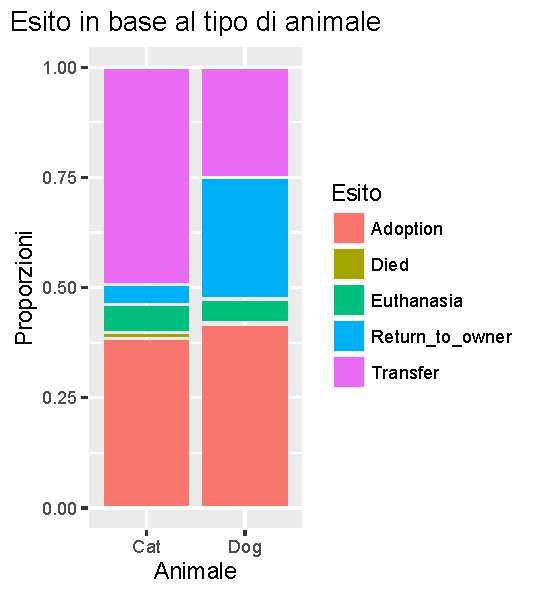
\includegraphics[width=0.4\textwidth]{./grafici/esito_animal.pdf}
	\caption{Esito in base al tipo di animale}\label{fig-animals}
\end{figure}

\subsection{Software utilizzato}

Nella realizzazione del progetto è stato utilizzato l'ambiente R in versione 3.2.4, esteso con alcune librerie:

\begin{itemize}
	\item \texttt{ggplot2}: per la rappresentazione dei grafici.
	\item \texttt{dplyr}: per la manipolazione dei dati.
	\item \texttt{nnet}: reti neurali e regressione logistica.
	\item \texttt{GAM}: GAM.
	\item \texttt{earth}: MARS.
	\item \texttt{randomForest}: random forest.
	\item \texttt{tree}: alberi di classificazione.
	\item \texttt{ada}: Boosting.
\end{itemize}

Tutte le librerie sono disponibili su CRAN mentre il codice del progetto è disponibile su GitHub all'indirizzo \url{https://github.com/GiacomoManzoli/AnimalShelter}.

\todo{aggiornare le librerie, manca quella del Bagging}
% !TEX encoding = UTF-8
% !TEX TS-program = pdflatex
% !TEX root = rel_datamining.tex
% !TEX spellcheck = it-IT

\section{Elaborazione delle variabili}

Il dataset si presenta con poche variabili che riassumono molte informazioni o che hanno un numero molto elevato di livelli. \`E quindi necessario andare ad estrapolare le informazioni da queste variabili, creandone di nuove e di più semplici.

\subsection{Il nome dell'animale}

La variabile \texttt{Name} ha più di 6000 possibili valori distinti e, ragionando a livello di previsione, sembra poco probabile che il nome dell'animale influisca sul suo destino. Tuttavia ci sono 7691 animali che non hanno un nome, questo probabilmente implica che si tratta di animali randagi che sono stati portati al rifugio\footnote{Non vengono fornite informazioni a riguardo} e quindi può essere meno probabile che il padrone li venga a recuperare. Analogamente se è stato trovato un'animale smarrito e con una targhetta con il nome al collo, è più probabile che il suo padrone vada a recuperarlo.

Il nome può quindi essere riassunto da una nuova variabile booleana \texttt{HasName} che specifica se l'animale ha un nome o meno.

Tracciando il grafico (Figura \ref{fig-has-name}) per visualizzare la ripartizione delle varie classi per la variabile risposta in base al valore di \texttt{HasName} si ha che le osservazioni fatte sembrano essere confermate dai dati: indipendentemente dal tipo di animale, se questo ha un nome è più probabile che venga recuperato dal suo padrone. Inoltre, si può notare anche che per i gatti, la probabilità di essere adottati è molto più alta se hanno un nome.

\begin{figure}[htbp]
	\centering
	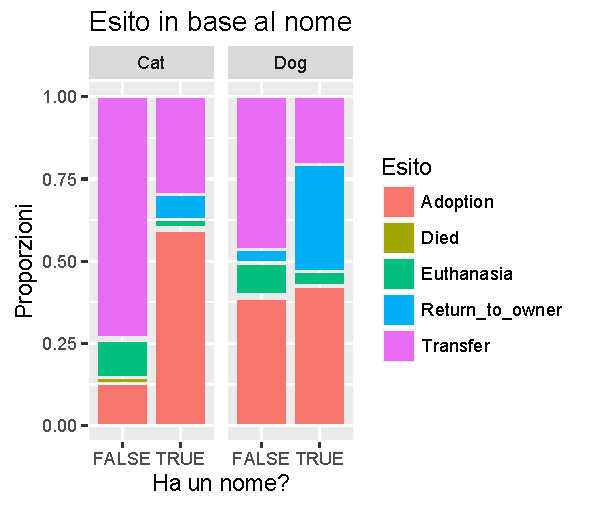
\includegraphics[width=0.5\textwidth]{./grafici/esito_has_name.pdf}
	\caption{Esito in base al nome}\label{fig-has-name}
\end{figure}

\subsection{La data di uscita}

Difficilmente la data in cui l'animale ha lasciato la struttura può tornare utile per effettuare previsioni future. Si possono però estrarre altre informazioni come la fascia oraria e il giorno della settimana in cui l'animale ha lasciato la struttura. 

Queste due informazioni possono tornare utili perché, ad esempio la gente nei week.end ha più tempo libero e quindi è più probabile che vada ad adottare un animale, oppure che per motivi logistici i trasferimenti possono essere fatti solamente la mattina.

Per estrapolare ciò vengono definite due nuove variabili \texttt{DayOfWeek} che assume come valore il giorno della settimana e \texttt{TimeOfDay} che può assumere come valori:

\begin{itemize}
	\item \textit{Mattina}: se l'ora è compresa tra le 6 e le 12.
	\item \textit{Pomeriggio}: se l'ora è compresa tra le 12 e le 17.
	\item \textit{Sera}: se l'ora è compresa tra le 17 e le 20.
	\item \textit{Notte}: per le restanti ore.
\end{itemize}

Come si può notare dal grafico (Figura \ref{fig-time}) c'è un picco sulle adozioni nella fascia serale. Sempre dal grafico si può notare che la notte sono più frequenti i trasferimenti, anche se la maggior parte di questi si viene svolta durante le ore diurne.

\begin{figure}[htbp]
	\centering
	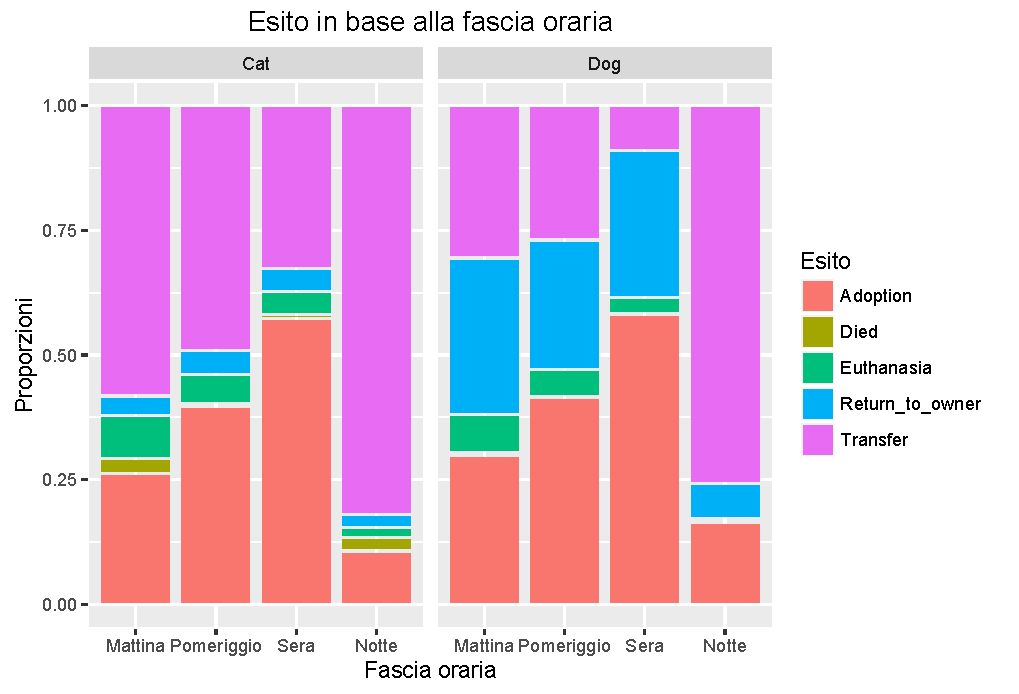
\includegraphics[width=0.6\textwidth]{./grafici/esito_time.pdf}
	\caption{Esito in base alla fascia oraria}\label{fig-time}
\end{figure}

Per quanto riguarda il giorno della settimana, dal grafico Figura \ref{fig-dow}, si può notare come le adozioni siano leggermente più probabili nel week-end.

\begin{figure}[htbp]
	\centering
	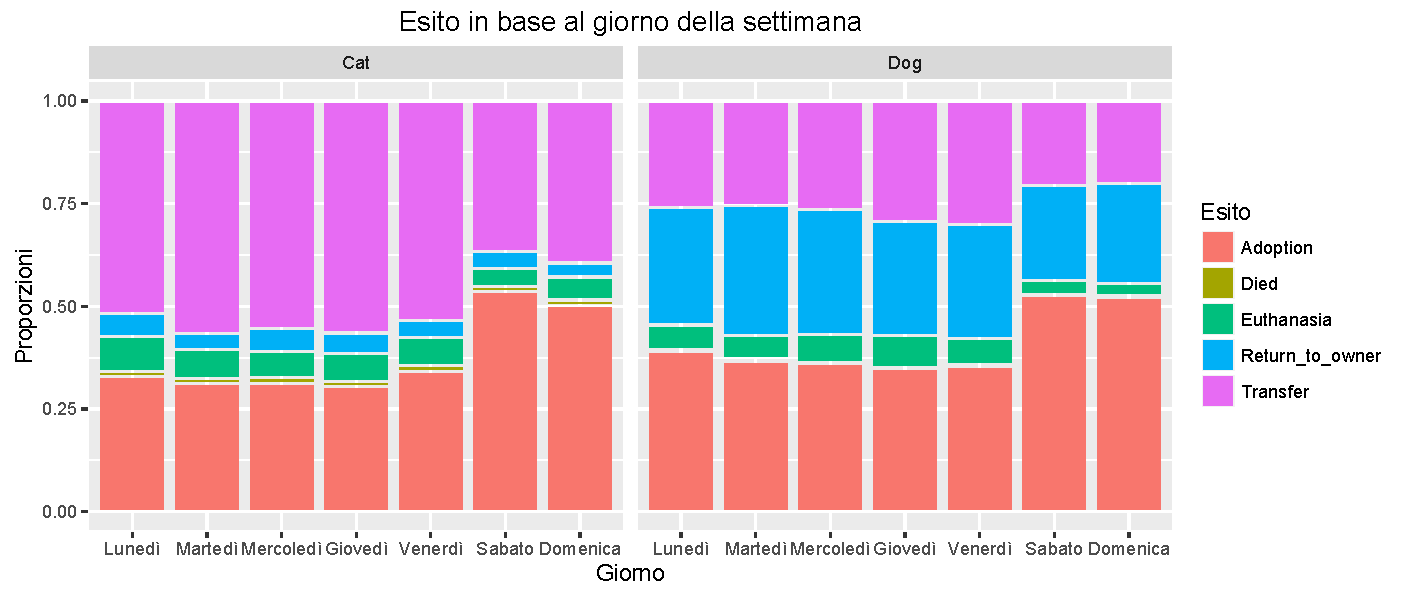
\includegraphics[width=0.9\textwidth]{./grafici/esito_week.pdf}
	\caption{Esito in base al giorno della settimana}\label{fig-dow}
\end{figure}

\subsection{Sesso e stato dell'animale}

La variabile \texttt{SexuponOutcome} prevede 6 possibili livelli che racchiudo l'informazione relativa al sesso e al fatto se l'animale è stato castrato o meno. C'è poi un livello \textit{Unknown} per gli animali per i quali non si hanno informazioni e in più ci sono dei valori non disponibili.

Questa variabile è stata quindi scomposta in \texttt{Gender} che specifica il sesso dell'animale e \texttt{Status}, che specifica se l'animale è stato castrato o meno. Entrambe le variabili hanno un terzo possibile valore \textit{Unknown} che rappresenta i dati non disponibili.

Dal grafico riportato in Fig \ref{fig-sesso-stato} si può notare che indipendentemente dal sesso e dal tipo di animale, se l'animale è stato castrato è più probabile che venga adottato. Se invece non è stato castrato oppure non ci sono informazioni a riguardo, è più probabile che venga trasferito.

\begin{figure}[htbp]
	\centering
	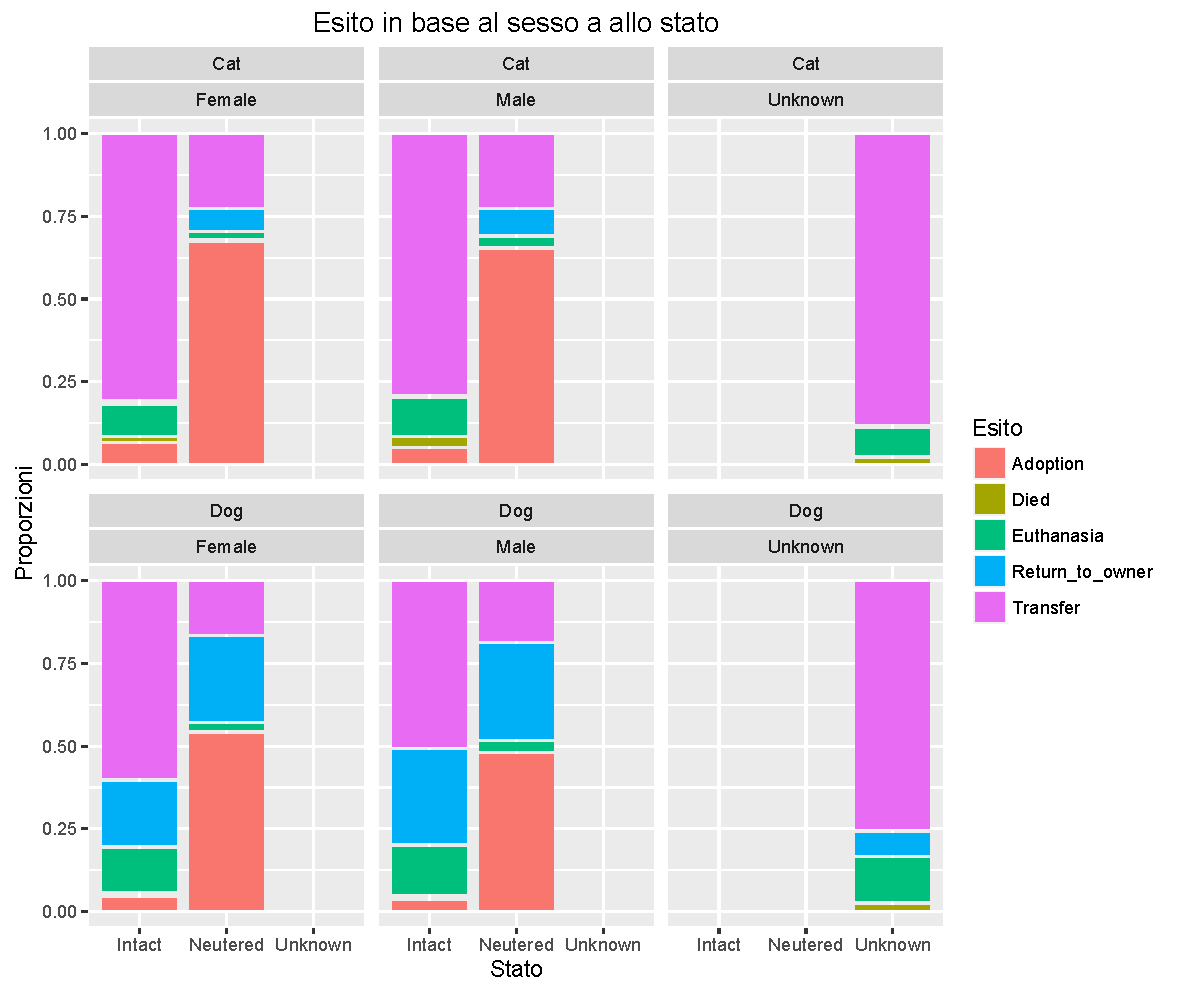
\includegraphics[width=0.8\textwidth]{./grafici/esito_sesso_stato.pdf}
	\caption{Esito in base al sesso e allo stato dell'animale}\label{fig-sesso-stato}
\end{figure}

\subsection{L'età dell'animale}

L'età dell'animale è memorizzata nella variabile \texttt{AgeuponOutcome} in un formato molto confusionale in quanto viene espressa come \textit{2 anni}, \textit{3 mesi}, ecc. Inoltre ci sono dei casi in cui alcuni valori non hanno la \textit{s} del plurale, ovvero tra i possibili valori della variabile ci sono ad esempio \textit{1 week} e \textit{1 weeks}, che quindi vengono considerati come valori distinti quando in realtà non lo sono.

La prima modifica è quindi quella di normalizzare i valori, esprimendoli con un numero intero che approssima l'età dell'animale espressa in giorni. Così facendo risulta più semplice classificare gli animali per fascia d'età. Infatti, si può assumere che un cucciolo è più probabile che venga adottato rispetto ad un animale più anziano, mentre gli animali troppo piccoli non possono essere adottati per legge.

Conviene quindi creare una nuova variabile \texttt{AgeCategory} con 5 possibili livelli:

\begin{itemize}
	\item \textit{Neonato}: da 0 a 29 giorni.
	\item \textit{Cucciolo}: da 30 a 365 giorni.
	\item \textit{Adulto}: da 366 a 3650 giorni (10 anni).
	\item \textit{Anziano}: più di dieci anni.
	\item \textit{Sconosciuta}.
\end{itemize}

Nella normalizzazione dei valori si è scelto di mantenere le 18 osservazioni con i valori mancati per l'età, marcandoli come sconosciuti, questo perché nel secondo dataset sono presenti delle osservazioni per le quali l'eta non è nota. Inoltre, si può ipotizzare che questi animali siano randagi e quindi che per questo motivo la loro eta non è nota.
Questa ipotesi deriva dal fatto che tra i possibili valori della variabile \texttt{OutcomeSubtype} c'è il valore \textit{SCRP} che indica un trasferimento relativo al programma di recupero dei gatti randagi\footnote{\url{http://www.maddiesfund.org/austin-animal-services-stray-cat-return-program.htm}} e quasi tutte le osservazioni con l'età mancante hanno proprio quel valore come \texttt{OutcomeSubtype}.

\begin{figure}[htbp]
	\centering
	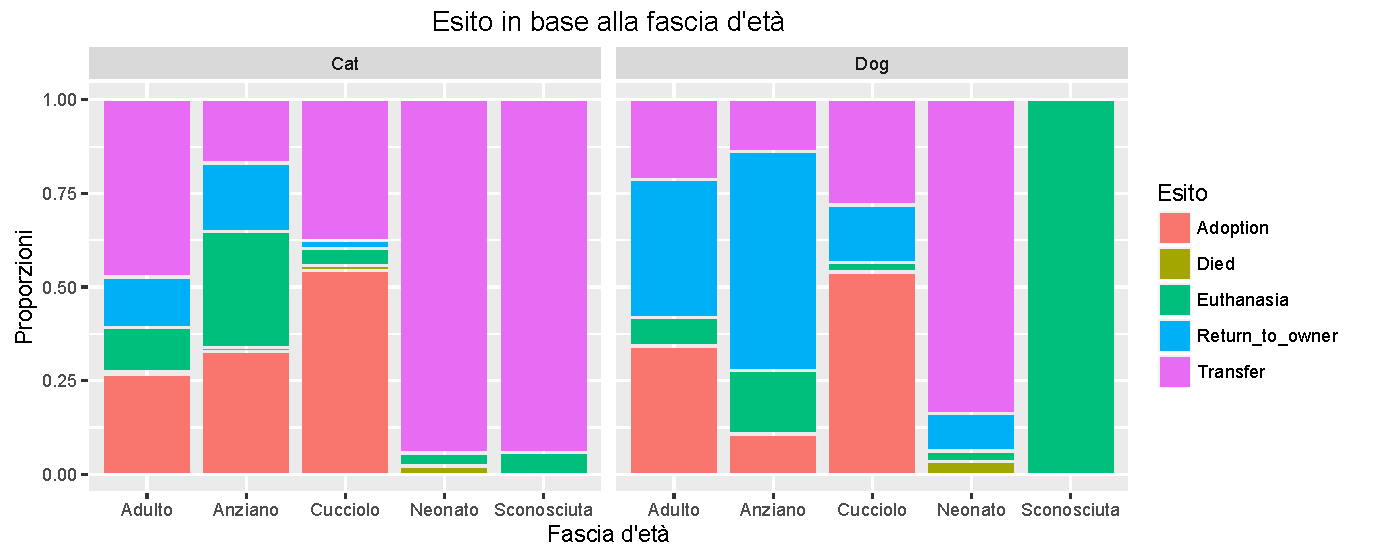
\includegraphics[width=0.9\textwidth]{./grafici/esito_eta.pdf}
	\caption{Esito in base alla fascia d'età dell'animale}\label{fig-eta}
\end{figure}

Come si può notare dal grafico Figura \ref{fig-eta}, nessuno degli animali neonati viene adottato ed è più probabile che vengano trasferiti. Per quanto riguarda la probabilità di adozione, questa è maggiore per i cuccioli e più bassa per i cani anziani. I gatti anziani hanno una maggiore probabilità di adozione rispetto ai cani anziani e questo può essere dovuto al fatto che la speranza di vita di un gatto è maggiore rispetto a quella di un cane.

\subsection{Razza}

Le informazioni relative alla razza dell'animale sono racchiuse nella variabile \texttt{Breed}, la quale ha 1340 possibili valori e specifica anche se l'animale è un incrocio o meno.

Osservando alcuni dei possibili valori, si può notare che se l'animale non è di razza, il valore della variabile comprende o due razze oppure la razza principale, seguita da \textit{Mix}. Si è scelto quindi di scomporre la variabile \texttt{Breed} nelle variabili \texttt{PrimaryBreed} (220 livelli), \texttt{SecondaryBreed} (144 livelli) e \texttt{IsMix} (booleana).

Ci sarebbero ulteriori informazioni che possono essere estratte da questa variabile, come la stazza dell'animale, la quale a sua volta va ad influire sull'aspettativa di vita e quindi sulla corretta classificazione della fascia d'età e sul carattere dell'animale. Tuttavia per estrarre queste informazioni in modo corretto è necessaria un'elevata conoscenza del dominio, ci si è quindi limitati alla scomposizione della variabile \texttt{Breed}.

\begin{figure}[htbp]
	\centering
	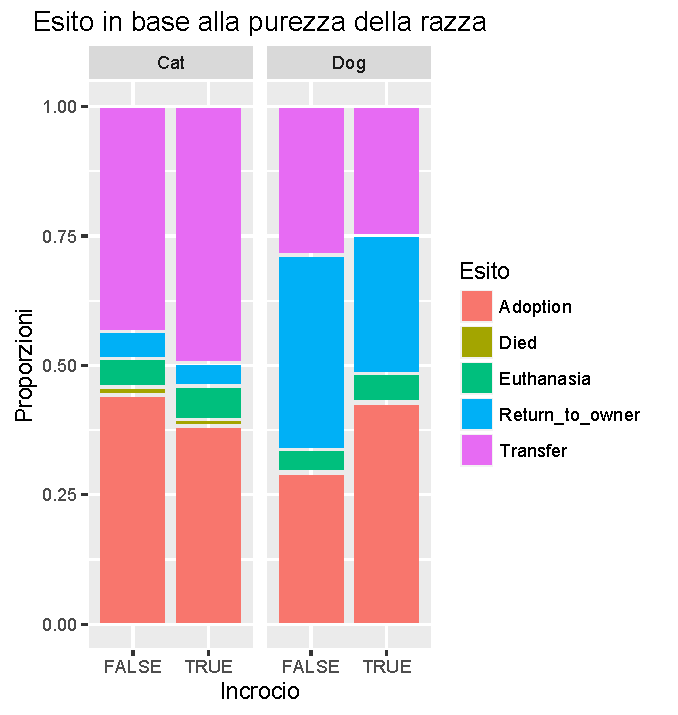
\includegraphics[width=0.5\textwidth]{./grafici/esito_mix.pdf}
	\caption{Esito in base alla fascia d'età dell'animale}\label{fig-mix}
\end{figure}


Come si può notare dal grafico in Figura \ref{fig-mix}, un cane di razza ha più probabilità di essere adottato rispetto ad un cane non di razza, mentre per i gatti sembra che avvenga il contrario. Non sono stati inseriti i grafici per le variabili \texttt{PrimaryBreed} e \texttt{SecondaryBreed} perché il numero elevato di possibili valori li rende incomprensibili.

\subsection{Colore}

Come per la razza, anche per il colore le informazioni sono racchiuse nell'unica variabile \texttt{Color} e, sempre come per la razza, queste informazioni sono state suddivise nelle variabili:

\begin{itemize}
	\item \texttt{PrimaryColor}: colore principale, 29 livelli.
	\item \texttt{SecondaryColor}: colore secondario, 24 livelli.
	\item \texttt{Pattern}: pattern del pelo, 10 livelli.
	\item \texttt{HasComplexColor}: valore booleano che specifica se il pelo dell'animale ha più colori o un certo pattern particolare.
\end{itemize}

Sarebbe poi necessario andare a normalizzare i valori dei colori, dato che ci sono più livelli che indicano lo stesso colore, come \textit{Orange} e \textit{Apricot} (albicocca), ma da una prima analisi grafica (Figura \ref{fig-colors}) sembra che, fissato il tipo di animale, le informazioni sul colore non influiscano sull'esito e in quei pochi casi che questo succede può essere dovuto al fatto che si hanno troppe poche osservazioni con quel determinato colore.

\begin{figure}[!ht]
	\centering
	\subfloat{%
		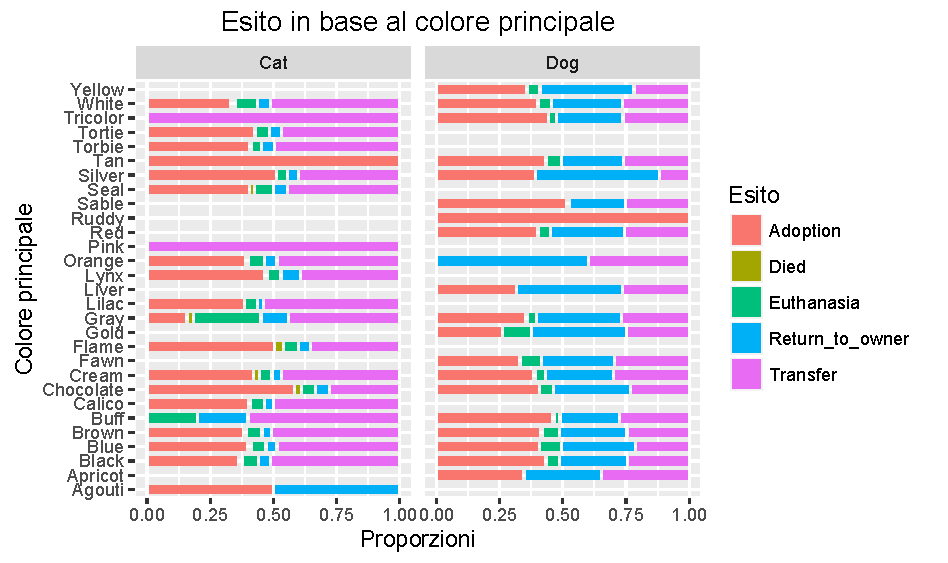
\includegraphics[width=0.48\textwidth]{./grafici/esito_colore_principale.pdf}
	}
	\quad
	\subfloat{%
		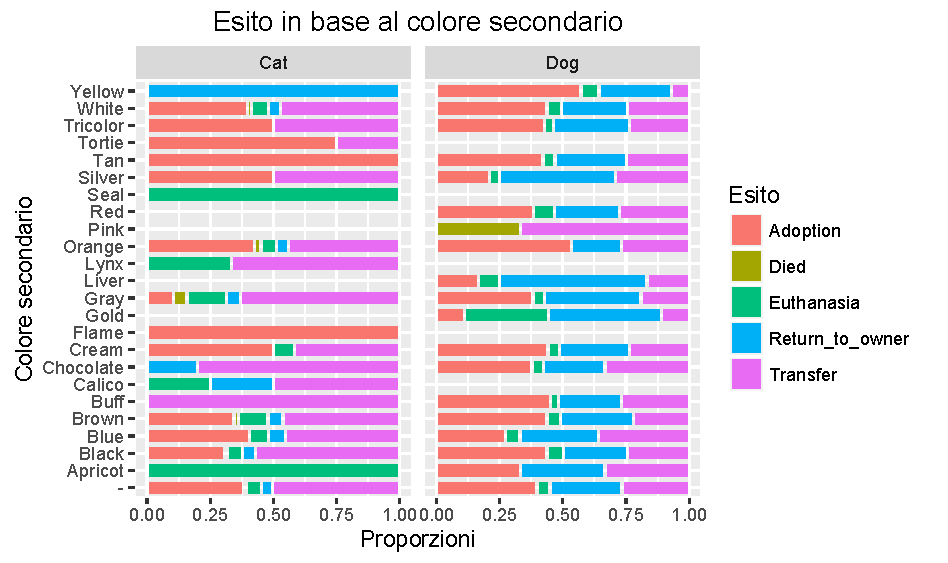
\includegraphics[width=0.48\textwidth]{./grafici/esito_colore_secondario.pdf}
	}
	
	\subfloat{%
		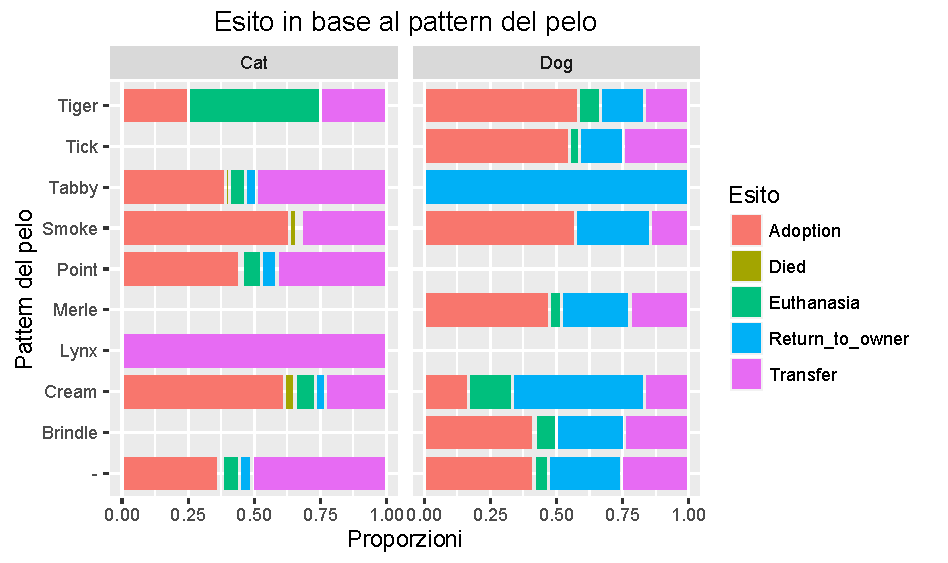
\includegraphics[width=0.48\textwidth]{./grafici/esito_pattern.pdf}
	}   
	\quad
	\subfloat{%
		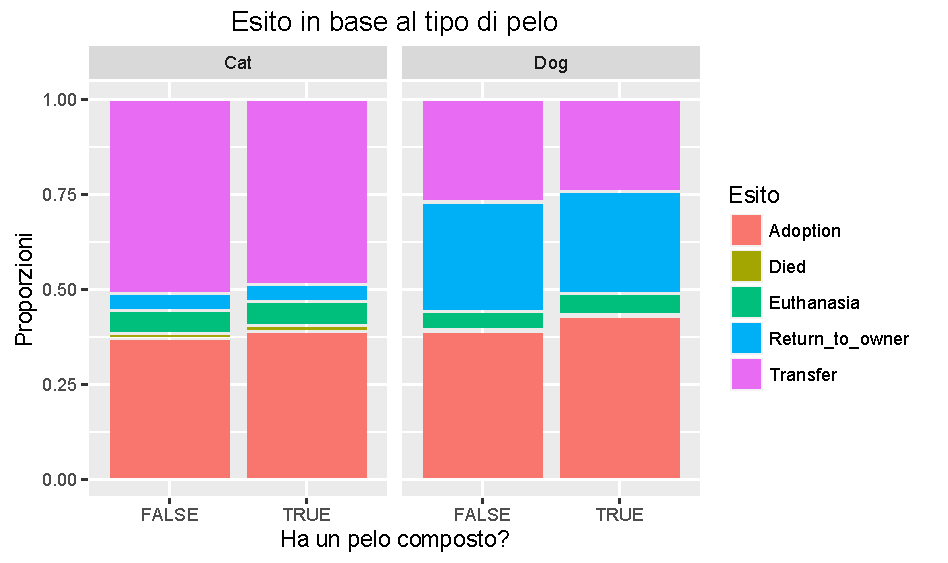
\includegraphics[width=0.48\textwidth]{./grafici/esito_has_complex_color.pdf}
	}
	\caption{I grafici della prima riga rappresentano rappresentano l'esito in base al colore principale e secondario. I grafici della seconda riga rappresentano l'esito in base al pattern e al fatto se il pelo dell'animale è composto o meno. Salvo alcuni casi dovuti al fatto che sono presenti poche osservazioni con quel determinato valore per una delle variabili, non si nota una correlazione tra il pelo e l'esito dell'animale una volta stabilito se si tratta di un cane o un gatto.}
	\label{fig-colors}
\end{figure}

\subsection{Riassunto delle trasformazioni}

Dopo aver applicato le trasformazioni precedentemente descritte ed aver eliminato le variabili \texttt{AnimalID} e \texttt{OutcomeSubtype}, il dataset ha assunto la seguente struttura:

\begin{verbatim}
'data.frame':	26711 obs. of  15 variables:
$ OutcomeType    : Factor w/ 5 levels "Adoption","Died",..
$ AnimalType     : Factor w/ 2 levels "Cat","Dog"
$ AgeCategory    : Factor w/ 4 levels "Adulto","Anziano",..
$ DayOfWeek      : Factor w/ 7 levels "Lunedì","Martedì",..
$ TimeOfDay      : Factor w/ 4 levels "Mattina","Pomeriggio",..
$ Gender         : Factor w/ 3 levels "Female","Male",..
$ Status         : Factor w/ 3 levels "Intact","Neutered",..
$ PrimaryColor   : Factor w/ 29 levels "Agouti","Apricot",..
$ SecondaryColor : Factor w/ 24 levels "-","Apricot",..
$ Pattern        : Factor w/ 10 levels "-","Brindle",..
$ HasComplexColor: Factor w/ 2 levels "FALSE","TRUE"
$ PrimaryBreed   : Factor w/ 220 levels "Abyssinian","Affenpinscher",..
$ SecondaryBreed : Factor w/ 144 levels "-","Affenpinscher",..
$ IsMix          : Factor w/ 2 levels "FALSE","TRUE"
$ HasName        : Factor w/ 2 levels "FALSE","TRUE"
\end{verbatim}
% !TEX encoding = UTF-8
% !TEX TS-program = pdflatex
% !TEX root = rel_datamining.tex
% !TEX spellcheck = it-IT

\section{Modelli}

Una volta trasformati i dati, sono stati provati vari modelli per vedere quale riesce ad effettuare le previsioni migliori.
In particolare sono stati utilizzati:

\begin{itemize}
	\item Regressione logistica multiclasse
	\item MARS
	\item GAM
	\item Alberi di classificazione
	\item Random Forest
	\item Reti Neurali
	\item Boosting
\end{itemize}

Per calcolare e confrontare i modelli, le 26000 osservazioni sono state suddivise in due insiemi, un insieme di validazione contenente il 20\% delle osservazioni e che viene utilizzato per confrontare gli errori commessi dai vari modelli e un altro set di dati composto dal restante 80\% delle osservazioni.

Le osservazioni di quest'ultimo set sono poi state suddivise in altri due sottoinsiemi, il \textit{test set} contenete il 20\% e il \textit{train set} contenente le restanti osservazioni. 

Con questa suddivisione è possibile utilizzare il \textit{train set} per calcolare il modello, provando più valori per gli eventuali iper-parametri, il \textit{test set} per stabilire quale configurazione di iper-parametri funziona meglio ed infine combinare i due set per calcolare la versione del modello da confrontare con gli altri modelli sui dati del \textit{validation set}.

Infine, una volta trovata la configurazione ottimale di ogni modello, questo viene ricalcolato anche sulla totalità delle osservazioni per poi essere utilizzato per effettuare le previsioni sul dataset secondario in modo da poterle caricare su Kaggle, ottenendo così un'ulteriore metrica per la valutazione della bontà del modello. 

Non è precisato su che cosa si basa il punteggio attribuito da Kaggle, tuttavia minore è il valore attribuito, migliore è il modello e per entrare nella top 100 dei punteggi migliori è necessario scendere sotto lo $0.7236$.

Per quanto riguarda le librerie contenenti le implementazioni dei vari modelli, si è cercato di utilizzare quelle viste a lezione, tuttavia non tutte queste librerie sono in grado di gestire la classificazione multiclasse e quindi è stato necessario cercare delle versioni alternative. Per i modelli GAM e Boosting, non sono state trovate librerie alternative, sono stati quindi utilizzati più modelli binomiali, combinati secondo la strategia \textit{one-vs-all}.

\subsection{Regressione logistica multiclasse}

Il primo modello utilizzato è stato quello che effettua la regressione logistica multiclasse. Tra le varie implementazioni della regressione logistica disponibili per R si è scelto di utilizzare \texttt{multinom} presente nel pacchetto \texttt{nnet}, la quale simula una regressione logistica utilizzando una rete neurale. 

\`E stata scelta questa particolare implementazione perché la funzione \texttt{glm} utilizzata in laboratorio funziona solo per la regressione binomiale e la funzione \texttt{mlogit} dell'omonimo pacchetto si è rilevata eccessivamente complessa. Si è comunque provato ad utilizzare \texttt{glm} combinando più modelli in modalità \textit{one-vs-all} (§\ref{sec-glm-glm}).

Il modello calcolato da \texttt{multinom} prevede, tra i vari iper-parametri, il valore di \texttt{decay} e confrontando l'effetto dei vari valori sul \textit{test set}, si è trovato come valore migliore $0.001$, il quale è stato utilizzato per calcolare il modello di regressione sulla versione combinata del \textit{test} e \textit{train set}, producendo un errore sul test di classificazione pari a $0.3365762$, ovvero circa del $33.66\%$.

Gli errori di classificazione sono riportati nella Tabella \ref{tab-reg}, dalla quale si può notare che la maggior parte degli errori commessi riguardano i trasferimenti che vengono classificati erroneamente come adozione. Un'altra cosa che si può notare è che nessuno degli animali viene classificato come deceduto per morte naturale e questo può essere causato dal fatto che nel dataset ci sono poche osservazioni che descrivono animali morti per cause naturali.

\begin{table}[htbp]
	\centering
		\begin{tabular}{cc|c|c|c|c|c|}
			\cline{3-7}
			&  & \multicolumn{5}{c|}{Valori osservati} \\ \cline{3-7} 
			&  & Adoption & Died & Euthanasia & Return to owner & Transfer \\ \hline
			\multicolumn{1}{|c|}{\multirow{5}{*}{\begin{tabular}[c]{@{}c@{}}Valori\\ predetti\end{tabular}}} & Adoption & 1827 & 1 & 38 & 364 & 462 \\ \cline{2-7} 
			\multicolumn{1}{|c|}{} & Died & 0 & 0 & 0 & 0 & 0 \\ \cline{2-7} 
			\multicolumn{1}{|c|}{} & Euthanasia & 3 & 1 & 40 & 17 & 21 \\ \cline{2-7} 
			\multicolumn{1}{|c|}{} & Return to owner & 242 & 4 & 71 & 446 & 142 \\ \cline{2-7} 
			\multicolumn{1}{|c|}{} & Transfer & 120 & 36 & 173 & 104 & 1233 \\ \hline
			\multicolumn{1}{l|}{}  & \multicolumn{1}{l|}{Errore classe (\%) } & 16.65& 100 & 87.57 & 52.09 & 33.63 \\ \cline{2-7}
		\end{tabular}%
	\caption{Errori di classificazione con il modello di regressione logistica.}
	\label{tab-reg}
\end{table}

Per quanto riguardo il punteggio ottenuto su Kaggle, il modello calcolato su tutto il dataset principale ha ottenuto un punteggio di $0.89358$.

\subsubsection{Regressione utilizzando \texttt{glm}}\label{sec-glm-glm}

Per effettuare la regressione logistica utilizzando \texttt{glm} è stato necessario calcolare 5 modelli, uno per ogni possibile valore della variabile risposta, e combinare tra loro le probabilità ottenute in modo da ottenere la classe più probabile per una determinata osservazione.

Con questo modello si è ottenuto un errore del $39.86\%$ e un punteggio su Kaggle di $0.87527$, anche se durante il calcolo del modello completo vengono sollevati dei warning rivelativi all'utilizzo di matrici con un rango troppo basso.

La Tabella \ref{tab-glm-mat} riporta le matrici di confusione per i 5 modelli binomiali, mentre la Tabella \ref{tab-glm} riporta il resoconto degli errori di classificazione. Da entrambe le tabelle è possibile notare come questo modello classifichi erroneamente molte osservazioni con la classe \textit{Died}, mentre la versione del pacchetto \texttt{multinom} non classifica nessuna osservazione con questa classe.

\begin{table}[htbp]
	\centering
	\subfloat[OutAdoption, errore: $0.217$]{%
		\hspace{.5cm}%
		\begin{tabular}{ll|l|l|}
			\cline{3-4}
			&     & \multicolumn{2}{l|}{Valori predetti} \\ \cline{3-4} 
			&     & No                & Yes              \\ \hline
			\multicolumn{1}{|l|}{\multirow{2}{*}{\begin{tabular}[c]{@{}l@{}}Valori\\ osservati\end{tabular}}} & No  & 2512             & 641             \\ \cline{2-4} 
			\multicolumn{1}{|l|}{}                                                                                                                                 & Yes & 522              & 1670             \\ \hline
		\end{tabular}
		\hspace{.5cm}%
	}\hspace{1cm}
	\subfloat[OutDied, errore: $0.108$]{%
		\hspace{.5cm}%
		\begin{tabular}{ll|l|l|}
			\cline{3-4}
			&     & \multicolumn{2}{l|}{Valori predetti} \\ \cline{3-4} 
			&     & No                & Yes              \\ \hline
			\multicolumn{1}{|l|}{\multirow{2}{*}{\begin{tabular}[c]{@{}l@{}}Valori\\ osservati\end{tabular}}} & No  & 4766             & 537             \\ \cline{2-4} 
			\multicolumn{1}{|l|}{}                                                                                                                                 & Yes & 40            & 2             \\ \hline
		\end{tabular}
		\hspace{.5cm}%
	}\hspace{1cm}
	\subfloat[OutEuthanasia, errore: $0.058$]{%
		\hspace{.5cm}%
		\begin{tabular}{ll|l|l|}
			\cline{3-4}
			&     & \multicolumn{2}{l|}{Valori predetti} \\ \cline{3-4} 
			&     & No                & Yes              \\ \hline
			\multicolumn{1}{|l|}{\multirow{2}{*}{\begin{tabular}[c]{@{}l@{}}Valori\\ osservati\end{tabular}}} & No  & 5008             & 15             \\ \cline{2-4} 
			\multicolumn{1}{|l|}{}                                                                                                                                 & Yes & 298              & 24            \\ \hline
		\end{tabular}
		\hspace{.5cm}%
	}\hspace{1cm}
	\subfloat[OutReturnToOwner, errore: $0.161$]{%
		\hspace{.5cm}%
		\begin{tabular}{ll|l|l|}
			\cline{3-4}
			&     & \multicolumn{2}{l|}{Valori predetti} \\ \cline{3-4} 
			&     & No                & Yes              \\ \hline
			\multicolumn{1}{|l|}{\multirow{2}{*}{\begin{tabular}[c]{@{}l@{}}Valori\\ osservati\end{tabular}}} & No  & 4279             & 135             \\ \cline{2-4} 
			\multicolumn{1}{|l|}{}                                                                                                                                 & Yes & 727              & 204             \\ \hline
		\end{tabular}
		\hspace{.5cm}%
	}\hspace{1cm}
	\subfloat[OutTransfer, errore: $0.196$]{%
		\hspace{.5cm}%
		\begin{tabular}{ll|l|l|}
			\cline{3-4}
			&     & \multicolumn{2}{l|}{Valori predetti} \\ \cline{3-4} 
			&     & No                & Yes              \\ \hline
			\multicolumn{1}{|l|}{\multirow{2}{*}{\begin{tabular}[c]{@{}l@{}}Valori\\ osservati\end{tabular}}} & No  & 3175             & 312             \\ \cline{2-4} 
			\multicolumn{1}{|l|}{}                                                                                                                                 & Yes & 738              & 1120             \\ \hline
		\end{tabular}
		\hspace{.5cm}%
	}\hspace{1cm}
	\caption{Matrici di confusione per i 5 classificatori con GLM}\label{tab-glm-mat}
\end{table}

\begin{table}[htbp]
	\centering
		\begin{tabular}{cc|c|c|c|c|c|}
			\cline{3-7}
			&  & \multicolumn{5}{c|}{Valori osservati} \\ \cline{3-7} 
			&  & Adoption & Died & Euthanasia & Return to owner & Transfer \\ \hline
			\multicolumn{1}{|c|}{\multirow{5}{*}{\begin{tabular}[c]{@{}c@{}}Valori\\ predetti\end{tabular}}} & Adoption & 1681 & 2 & 43 & 344 & 455 \\ \cline{2-7} 
			\multicolumn{1}{|c|}{} & Died & 238 & 2 & 29 & 124 & 120 \\ \cline{2-7} 
			\multicolumn{1}{|c|}{} & Euthanasia & 0 & 1 & 17 & 4 & 11 \\ \cline{2-7} 
			\multicolumn{1}{|c|}{} & Return to owner & 184 & 2 & 59 & 362 & 120 \\ \cline{2-7} 
			\multicolumn{1}{|c|}{} & Transfer & 89 & 35 & 174 & 97 & 1152 \\ \hline
			\multicolumn{1}{l|}{}  & \multicolumn{1}{l|}{Errore classe (\%) } & 23.31& 95.23 & 94.72 & 61.11 & 37.66 \\ \cline{2-7}
		\end{tabular}%
	\caption{Errori di classificazione con GLM.}
	\label{tab-glm}
\end{table}

\subsection{MARS}

Come modello MARS è stato utilizzato quello disponibile nel pacchetto \texttt{earth} con la configurazione di default.

Così facendo si è ottenuto un errore del $36.40\%$ e un punteggio su Kaggle di $0.9001$.

Anche in questo caso, come si può notare dalla Tabella \ref{tab-mars}, il modello non ha classificato nessuna delle osservazioni come \textit{Died} o \textit{Euthanasia}.

\begin{table}[htbp]
	\centering

		\begin{tabular}{cc|c|c|c|c|c|}
			\cline{3-7}
			&  & \multicolumn{5}{c|}{Valori osservati} \\ \cline{3-7} 
			&  & Adoption & Died & Euthanasia & Return to owner & Transfer \\ \hline
			\multicolumn{1}{|c|}{\multirow{5}{*}{\begin{tabular}[c]{@{}c@{}}Valori\\ predetti\end{tabular}}} & Adoption & 1994 & 2 & 61 & 599 & 566 \\ \cline{2-7} 
			\multicolumn{1}{|c|}{} & Died & 0 & 0 & 0 & 0 & 2 \\ \cline{2-7} 
			\multicolumn{1}{|c|}{} & Euthanasia & 0 & 0 & 0 & 0 & 0 \\ \cline{2-7} 
			\multicolumn{1}{|c|}{} & Return to owner & 99 & 2 & 48 & 187 & 74 \\ \cline{2-7} 
			\multicolumn{1}{|c|}{} & Transfer & 99 & 38 & 213 & 145 & 1218 \\ \hline
			\multicolumn{1}{l|}{}  & \multicolumn{1}{l|}{Errore classe (\%) } & 9.03& 100 & 100 & 79.91 & 34.44 \\ \cline{2-7}
		\end{tabular}%
	
	\caption{Errori di classificazione con MARS.}
	\label{tab-mars}
\end{table}

\subsection{GAM}

Il modello GAM è stato calcolato utilizzando la funzione \texttt{gam} dell'omonimo pacchetto e selezionando tutte le variabili a disposizione.

Dal momento che GAM utilizza come predittore un modello lineare generalizzato e che non è stato possibile utilizzare le spline di lisciamento perché tutte le variabili sono qualitative, i risultati ottenuti con questo modello sono molto simili a quelli ottenuti con il modello lineare generalizzato riportato in §\ref{sec-glm-glm}.

Sempre come per il modello della regressione logistica, non è stato possibile calcolare un unico modello, ma è stato necessario definire 5 modelli, uno per ogni possibile valore della variabile risposta, per poi classificare l'osservazione utilizzando la classe più probabile.

Così facendo si è ottenuto un errore di classificazione del $34.03\%$ sul test di validazione e un punteggio di $0.87405$ su Kaggle.

Gli errori di classificazione vengono riportati nelle tabelle \ref{tab-gam-matrix} e \ref{tab-gam}. 
Dalla prima tabella è possibile osservare come il modello \texttt{OutDied} non classifichi nessuna osservazione come positiva, ottenendo comunque un errore molto basso a causa del numero limitato di osservazioni che compaiono nel training set che hanno quella determinata classe. 

\begin{table}[htbp]
	\centering
	\subfloat[OutAdoption, errore: $0.217$]{%
		\hspace{.5cm}%
		\begin{tabular}{ll|l|l|}
			\cline{3-4}
			&     & \multicolumn{2}{l|}{Valori predetti} \\ \cline{3-4} 
			&     & No                & Yes              \\ \hline
			\multicolumn{1}{|l|}{\multirow{2}{*}{\begin{tabular}[c]{@{}l@{}}Valori\\ osservati\end{tabular}}} & No  & 2512             & 641             \\ \cline{2-4} 
			\multicolumn{1}{|l|}{}                                                                                                                                 & Yes & 522              & 1670             \\ \hline
		\end{tabular}
		\hspace{.5cm}%
	}\hspace{1cm}
	\subfloat[OutDied, errore: $0.007$]{%
		\hspace{.5cm}%
		\begin{tabular}{ll|l|l|}
			\cline{3-4}
			&     & \multicolumn{2}{l|}{Valori predetti} \\ \cline{3-4} 
			&     & No                & Yes              \\ \hline
			\multicolumn{1}{|l|}{\multirow{2}{*}{\begin{tabular}[c]{@{}l@{}}Valori\\ osservati\end{tabular}}} & No  & 5303             & 0             \\ \cline{2-4} 
			\multicolumn{1}{|l|}{}                                                                                                                                 & Yes & 42            & 0             \\ \hline
		\end{tabular}
		\hspace{.5cm}%
	}\hspace{1cm}
	\subfloat[OutEuthanasia, errore: $0.058$]{%
		\hspace{.5cm}%
		\begin{tabular}{ll|l|l|}
			\cline{3-4}
			&     & \multicolumn{2}{l|}{Valori predetti} \\ \cline{3-4} 
			&     & No                & Yes              \\ \hline
			\multicolumn{1}{|l|}{\multirow{2}{*}{\begin{tabular}[c]{@{}l@{}}Valori\\ osservati\end{tabular}}} & No  & 5008             & 15             \\ \cline{2-4} 
			\multicolumn{1}{|l|}{}                                                                                                                                 & Yes & 298              & 24            \\ \hline
		\end{tabular}
		\hspace{.5cm}%
	}\hspace{1cm}
	\subfloat[OutReturnToOwner, errore: $0.161$]{%
		\hspace{.5cm}%
		\begin{tabular}{ll|l|l|}
			\cline{3-4}
			&     & \multicolumn{2}{l|}{Valori predetti} \\ \cline{3-4} 
			&     & No                & Yes              \\ \hline
			\multicolumn{1}{|l|}{\multirow{2}{*}{\begin{tabular}[c]{@{}l@{}}Valori\\ osservati\end{tabular}}} & No  & 4279             & 135             \\ \cline{2-4} 
			\multicolumn{1}{|l|}{}                                                                                                                                 & Yes & 727              & 204             \\ \hline
		\end{tabular}
		\hspace{.5cm}%
	}\hspace{1cm}
	\subfloat[OutTransfer, errore: $0.196$]{%
		\hspace{.5cm}%
		\begin{tabular}{ll|l|l|}
			\cline{3-4}
			&     & \multicolumn{2}{l|}{Valori predetti} \\ \cline{3-4} 
			&     & No                & Yes              \\ \hline
			\multicolumn{1}{|l|}{\multirow{2}{*}{\begin{tabular}[c]{@{}l@{}}Valori\\ osservati\end{tabular}}} & No  & 3175             & 312             \\ \cline{2-4} 
			\multicolumn{1}{|l|}{}                                                                                                                                 & Yes & 738              & 1120             \\ \hline
		\end{tabular}
		\hspace{.5cm}%
	}\hspace{1cm}
	\caption{Matrici di confusione per i 5 classificatori con GAM}\label{tab-gam-matrix}
\end{table}

\begin{table}[htbp]
	\centering
		\begin{tabular}{cc|c|c|c|c|c|}
			\cline{3-7}
			&  & \multicolumn{5}{c|}{Valori osservati} \\ \cline{3-7} 
			&  & Adoption & Died & Euthanasia & Return to owner & Transfer \\ \hline
			\multicolumn{1}{|c|}{\multirow{5}{*}{\begin{tabular}[c]{@{}c@{}}Valori\\ predetti\end{tabular}}} & Adoption & 1878 & 2 & 49 & 394 & 493 \\ \cline{2-7} 
			\multicolumn{1}{|c|}{} & Died & 0 & 0 & 0 & 0 & 0 \\ \cline{2-7} 
			\multicolumn{1}{|c|}{} & Euthanasia & 1 & 1 & 17 & 4 & 11 \\ \cline{2-7} 
			\multicolumn{1}{|c|}{} & Return to owner & 213 & 2 & 67 & 415 & 138 \\ \cline{2-7} 
			\multicolumn{1}{|c|}{} & Transfer & 100 & 37 & 189 & 118 & 1216 \\ \hline
			\multicolumn{1}{l|}{}  & \multicolumn{1}{l|}{Errore classe (\%) } & 14.32& 100 & 94.72 & 55.42 & 34.55 \\ \cline{2-7}
		\end{tabular}%
	\caption{Errori di classificazione con GAM.}
	\label{tab-gam}
\end{table}

\subsection{Alberi di classificazione}

Per calcolare l'albero di classificazione è stato utilizzato il modello disponibile nel pacchetto \texttt{tree}.

L'albero è stato costruito utilizzando le osservazioni presenti nel \textit{train set}, espandendolo fino ad ottenere una devianza interna alle foglie minore di $0.002$ (\texttt{mindev=0.002}). 
Dopodiché sono stati usati i dati del \textit{test set} per potare l'albero in modo da limitare l'overfitting, ottenendo come albero migliore quello con 21 foglie.

L'albero così prodotto ha ottenuto un errore di classificazione del $35.43\%$, ovvero leggermente peggiore rispetto alla regressione logistica.

La Tabella \ref{tab-tree} riporta gli errori di classificazione commessi dal modello, per i quali valgono le stesse considerazioni fatte per la regressione logistica, alle quali si aggiunge il fatto che anche la classe \textit{Euthanasia} non viene mai assegnata.

Questo fatto può essere osservato andando ad effettuare il \texttt{plot} dell'albero ottenuto, dal quale è possibile osservare come nessuna foglia dell'albero abbia etichetta \textit{Died} o \textit{Euthanasia}\footnote{Il plot dell'albero è stato omesso perché è troppo grande rispetto alle dimensioni del documento}.

C'è però da tenere in considerazione che questo modello è stato calcolato senza utilizzare le variabili \texttt{PrimaryBreed} e \texttt{SecondaryBreed} perché con la funzione \texttt{tree} non è possibile usare variabili di tipo \texttt{Factor} con più di 32 livelli ed entrambe le variabili sforavano questo limite. Nonostante ciò il punteggio ottenuto su Kaggle è di $0.87657$, ovvero migliore rispetto a quello ottenuto dalla regressione logistica.

\begin{table}[htbp]
	\centering
		\begin{tabular}{cc|c|c|c|c|c|}
			\cline{3-7}
			&  & \multicolumn{5}{c|}{Valori osservati} \\ \cline{3-7} 
			&  & Adoption & Died & Euthanasia & Return to owner & Transfer \\ \hline
			\multicolumn{1}{|c|}{\multirow{5}{*}{\begin{tabular}[c]{@{}c@{}}Valori\\ predetti\end{tabular}}} & Adoption & 1765 & 2 & 33 & 352 & 431 \\ \cline{2-7} 
			\multicolumn{1}{|c|}{} & Died & 0 & 0 & 0 & 0 & 0 \\ \cline{2-7} 
			\multicolumn{1}{|c|}{} & Euthanasia & 0 & 0 & 0 & 0 & 0 \\ \cline{2-7} 
			\multicolumn{1}{|c|}{} & Return to owner & 289 & 3 & 86 & 465 & 206 \\ \cline{2-7} 
			\multicolumn{1}{|c|}{} & Transfer & 138 & 37 & 203 & 114 & 1221 \\ \hline
			\multicolumn{1}{l|}{}  & \multicolumn{1}{l|}{Errore classe (\%) } & 19.47& 100 & 100 & 52.05 & 34.28 \\ \cline{2-7}
		\end{tabular}%
	\caption{Errori di classificazione con l'albero di classificazione.}
	\label{tab-tree}
\end{table}

\subsection{Random Forest}

Un miglioramento al modello degli alberi di classificazione è dato dal modello delle random forest, le quali effettuano la classificazione combinando più alberi di dimensioni ridotte.

Trattandosi di una combinazione di alberi di classificazione, anche questo modello soffre del problema relativo alle variabili \texttt{PrimaryBreed} e \texttt{SecondaryBreed}, le quali sono state scartate dal dataset.

I parametri del modello che si sono rivelati essere migliori sono \texttt{mtry} uguale a 12 e \texttt{ntree} uguale a 600, ovvero la configurazione migliore della foresta ha 600 alberi di classificazione, addestrati su un set ridotto delle osservazioni e utilizzando tutte e 12 le variabili a disposizione. Infatti, il parametro \texttt{mtry} specifica il numero di variabili da scegliere a caso tra quelle disponibili quando viene estratto un campione per calcolare un singolo albero.
Gli altri valori provati per \texttt{mtry} sono stati 5 e 10, ma hanno prodotto risultati peggiori.

Con questa configurazione, il modello ha ottenuto un errore di classificazione del $18.63\%$ sul set di validazione, tuttavia il punteggio calcolato da Kaggle risulta essere $2.1834$.

Come prima causa di questa discrepanza si è pensato all'\textit{overfitting} dei dati da parte della foresta. Tuttavia, le due metriche sono state calcolate su una porzione del dataset che non è stata utilizzata per calcolare il modello e quindi l'overfitting dovrebbe aver fatto aumentare anche l'errore di classificazione sul set di validazione.

Un'altra possibile causa deriva dal fatto che Kaggle sembra penalizzare maggiormente le previsioni certe, ovvero quello che danno probabilità 1 ad una determinata classe e si è notato che il modello ha effettuato circa il $10\%$ di previsione certe per le classi \textit{Adoption} e \textit{Transfer}.

\begin{table}[htbp]
	\centering
		\begin{tabular}{cc|c|c|c|c|c|}
			\cline{3-7}
			&  & \multicolumn{5}{c|}{Valori osservati} \\ \cline{3-7} 
			&  & Adoption & Died & Euthanasia & Return to owner & Transfer \\ \hline
			\multicolumn{1}{|c|}{\multirow{5}{*}{\begin{tabular}[c]{@{}c@{}}Valori\\ predetti\end{tabular}}} & Adoption & 1961 & 3 & 27 & 224 & 259 \\ \cline{2-7} 
			\multicolumn{1}{|c|}{} & Died & 0 & 29 & 0 & 0 & 2 \\ \cline{2-7} 
			\multicolumn{1}{|c|}{} & Euthanasia & 4 & 1 & 203 & 7 & 15 \\ \cline{2-7} 
			\multicolumn{1}{|c|}{} & Return to owner & 141 & 2 & 29 & 646 & 72 \\ \cline{2-7} 
			\multicolumn{1}{|c|}{} & Transfer & 86 & 7 & 63 & 54 & 1510 \\ \hline
			\multicolumn{1}{l|}{}  & \multicolumn{1}{l|}{Errore classe (\%) } & 10.53& 30.95 & 36.95 & 30.61 & 18.72 \\ \cline{2-7}
		\end{tabular}%
	\caption{Errori di classificazione con random forest.}
	\label{tab-forest}
\end{table}



\subsection{Reti neurali}

Come modello di una rete neurale è stato utilizzato quello disponibile nel pacchetto \texttt{nnet}, il quale permette di impostare alcuni iper-parametri come:

\begin{itemize}
	\item \texttt{MaxNWts}: massimo numero di pesi nella rete. Impostato a 10000 perché il valore di default è troppo basso rispetto al numero di variabili.
	\item \texttt{maxit}: massimo numero di iterazioni nell'addestramento della rete. Durante l'ottimizzazione dei parametri è stato mantenuto fissato a 200, mentre per i due modelli finali è stato portato a 1000.
	\item \texttt{decay}: fattore di decadimento dei pesi per l'algoritmo di addestramento. Impostato a $0.001668$, valore individuato utilizzando i dati del \textit{train} e \textit{test set}.
	\item \texttt{size}: numero di nodi presenti nello strato nascosto della rete. Impostato a 10 dal momento che non c'è un modo sistematico per stabilire il numero ottimale ed effettuare l'ottimizzazione di questo iper-parametro richiede troppo tempo.
\end{itemize}

La rete così ottenuta ha prodotto un errore di classificazione del $29,31\%$, senza mai prevedere la morte naturale per gli animali, e un punteggio di $0.93989$ su Kaggle.
La Tabella \ref{tab-net} riporta più in dettaglio gli errori commessi dalla rete.

\begin{table}[htbp]
	\centering
		\begin{tabular}{cc|c|c|c|c|c|}
			\cline{3-7}
			&  & \multicolumn{5}{c|}{Valori osservati} \\ \cline{3-7} 
			&  & Adoption & Died & Euthanasia & Return to owner & Transfer \\ \hline
			\multicolumn{1}{|c|}{\multirow{5}{*}{\begin{tabular}[c]{@{}c@{}}Valori\\ predetti\end{tabular}}} & Adoption & 1892 & 4 & 41 & 338 & 375 \\ \cline{2-7} 
			\multicolumn{1}{|c|}{} & Died & 0 & 0 & 0 & 0 & 0 \\ \cline{2-7} 
			\multicolumn{1}{|c|}{} & Euthanasia & 2 & 1 & 63 & 8 & 20 \\ \cline{2-7} 
			\multicolumn{1}{|c|}{} & Return to owner & 188 & 1 & 70 & 495 & 135 \\ \cline{2-7} 
			\multicolumn{1}{|c|}{} & Transfer & 110 & 36 & 148 & 90 & 1328 \\ \hline
			\multicolumn{1}{l|}{}  & \multicolumn{1}{l|}{Errore classe (\%) } & 13.68& 100 & 80.43 & 46.83 & 28.52 \\ \cline{2-7}
		\end{tabular}%
	\caption{Errori di classificazione con la rete neurale.}
	\label{tab-net}
\end{table}

\subsection{Boosting}

Come modello di Boosting è stata utilizzata la versione di default della libreria \texttt{ada} e dal momento che con questo modello non è possibile effettuare la classificazione multiclasse, è stato necessario adottare la stessa strategia utilizzata per il GAM e per la regressione logistica.

Sono stati quindi calcolati 5 modelli, uno per ogni possibile valore della variabile risposta e combinati tra loro per produrre la previsione finale. 

Le matrici di confusione dei vari modelli sono riportate nella Tabella \ref{tab-boost-mat} mentre la Tabella \ref{tab-boost} contiene gli errori di classificazione.

Dalla matrice di confusione del modello \texttt{OutDied} si può notare che, anche se non viene mai prevista la classe \textit{Died}, l'errore commesso è minimo e questo è causato dal fatto che nel dataset completo, le osservazioni con questa classe sono in netta minoranza rispetto le altre.

L'errore totale commesso dal modello è del $32,61\%$ e il punteggio ottenuto su Kaggle è di $0.88321$.

\begin{table}[htbp]
\centering
\subfloat[OutAdoption, errore: $0.215$]{%
	\hspace{.5cm}%
	\begin{tabular}{ll|l|l|}
		\cline{3-4}
		&     & \multicolumn{2}{l|}{Valori predetti} \\ \cline{3-4} 
		&     & No                & Yes              \\ \hline
		\multicolumn{1}{|l|}{\multirow{2}{*}{\begin{tabular}[c]{@{}l@{}}Valori\\ osservati\end{tabular}}} & No  & 2494             & 659             \\ \cline{2-4} 
		\multicolumn{1}{|l|}{}                                                                                                                                 & Yes & 495              & 1697             \\ \hline
	\end{tabular}
	\hspace{.5cm}%
}\hspace{1cm}
\subfloat[OutDied, errore: $0.007$]{%
	\hspace{.5cm}%
	\begin{tabular}{ll|l|l|}
		\cline{3-4}
		&     & \multicolumn{2}{l|}{Valori predetti} \\ \cline{3-4} 
		&     & No                & Yes              \\ \hline
		\multicolumn{1}{|l|}{\multirow{2}{*}{\begin{tabular}[c]{@{}l@{}}Valori\\ osservati\end{tabular}}} & No  & 5303             & 0             \\ \cline{2-4} 
		\multicolumn{1}{|l|}{}                                                                                                                                 & Yes & 42            & 0             \\ \hline
	\end{tabular}
	\hspace{.5cm}%
}\hspace{1cm}
\subfloat[OutEuthanasia, errore: $0.057$]{%
	\hspace{.5cm}%
	\begin{tabular}{ll|l|l|}
		\cline{3-4}
		&     & \multicolumn{2}{l|}{Valori predetti} \\ \cline{3-4} 
		&     & No                & Yes              \\ \hline
		\multicolumn{1}{|l|}{\multirow{2}{*}{\begin{tabular}[c]{@{}l@{}}Valori\\ osservati\end{tabular}}} & No  & 5019             & 4             \\ \cline{2-4} 
		\multicolumn{1}{|l|}{}                                                                                                                                 & Yes & 302              & 20             \\ \hline
	\end{tabular}
	\hspace{.5cm}%
}\hspace{1cm}
\subfloat[OutReturnToOwner, errore: $0.163$]{%
	\hspace{.5cm}%
	\begin{tabular}{ll|l|l|}
		\cline{3-4}
		&     & \multicolumn{2}{l|}{Valori predetti} \\ \cline{3-4} 
		&     & No                & Yes              \\ \hline
		\multicolumn{1}{|l|}{\multirow{2}{*}{\begin{tabular}[c]{@{}l@{}}Valori\\ osservati\end{tabular}}} & No  & 4293             & 121             \\ \cline{2-4} 
		\multicolumn{1}{|l|}{}                                                                                                                                 & Yes & 752              & 179             \\ \hline
	\end{tabular}
	\hspace{.5cm}%
}\hspace{1cm}
\subfloat[OutTransfer, errore: $0.192$]{%
	\hspace{.5cm}%
	\begin{tabular}{ll|l|l|}
		\cline{3-4}
		&     & \multicolumn{2}{l|}{Valori predetti} \\ \cline{3-4} 
		&     & No                & Yes              \\ \hline
		\multicolumn{1}{|l|}{\multirow{2}{*}{\begin{tabular}[c]{@{}l@{}}Valori\\ osservati\end{tabular}}} & No  & 3220             & 267             \\ \cline{2-4} 
		\multicolumn{1}{|l|}{}                                                                                                                                 & Yes & 763              & 1095             \\ \hline
	\end{tabular}
	\hspace{.5cm}%
}\hspace{1cm}
\caption{Matrici di confusione per i 5 classificatori con Boosting}\label{tab-boost-mat}
\end{table}

\begin{table}[htbp]
	\centering
		\begin{tabular}{cc|c|c|c|c|c|}
			\cline{3-7}
			&  & \multicolumn{5}{c|}{Valori osservati} \\ \cline{3-7} 
			&  & Adoption & Died & Euthanasia & Return to owner & Transfer \\ \hline
			\multicolumn{1}{|c|}{\multirow{5}{*}{\begin{tabular}[c]{@{}c@{}}Valori\\ predetti\end{tabular}}} & Adoption & 1900 & 4 & 53 & 393 & 475 \\ \cline{2-7} 
			\multicolumn{1}{|c|}{} & Died & 0 & 0 & 0 & 0 & 0 \\ \cline{2-7} 
			\multicolumn{1}{|c|}{} & Euthanasia & 1 & 0 & 17 & 3 & 4 \\ \cline{2-7} 
			\multicolumn{1}{|c|}{} & Return to owner & 185 & 1 & 70 & 437 & 131 \\ \cline{2-7} 
			\multicolumn{1}{|c|}{} & Transfer & 106 & 37 & 182 & 98 & 1248 \\ \hline
			\multicolumn{1}{l|}{}  & \multicolumn{1}{l|}{Errore classe (\%) } & 13.32& 100 & 94.72 & 53.06 & 32.83 \\ \cline{2-7}
		\end{tabular}%
	\caption{Errori di classificazione con Boosting.}
	\label{tab-boost}
\end{table}



% !TEX encoding = UTF-8
% !TEX TS-program = pdflatex
% !TEX root = rel_datamining.tex
% !TEX spellcheck = it-IT

\section{Conclusioni}

\subsection{Riepilogo}

I risultati ottenuti dai vari modelli sono riportati in Tabella \ref{tab-riepilogo} e come si può notare, il modello migliore che ha ottenuto un errore minore è quello delle random forest, anche se il punteggio che ha ottenuto su Kaggle è quello peggiore.
Il miglior modello secondo Kaggle è il GAM, che sulla classifica provvisoria del sito si trova in posizione 480 su 876.

\begin{table}[htbp]
	\centering
	\begin{tabular}{|c|c|c|c|}
		\hline
		Modello & Variante & \begin{tabular}[c]{@{}c@{}}Errore di\\ classificazione (\%)\end{tabular} & \begin{tabular}[c]{@{}c@{}}Punteggio su\\ Kaggle\end{tabular} \\ \hline
		\multirow{2}{*}{GLM}& \texttt{multinom} & 33.66 & 0.89358 \\ \cline{2-4}
		& \texttt{glm} & 39.86 & 0.87527 \\ \hline
		MARS & - & 36.40 & 0.90010 \\ \hline
		GAM & - & 34.04 & 0.87405 \\ \hline
		Albero & - & 35.43 & 0.87657 \\ \hline
		\begin{tabular}[c]{@{}c@{}}Random\\ Forest\end{tabular} & - & 18.63 & 2.1834 \\ \hline
		Rete neurale & - & 29.31 & 0.93989 \\ \hline
		Boosting & - & 32.61 & 0.88321 \\ \hline
	\end{tabular}
	\caption{Riepilogo dei risultati ottenuti con i vari modelli.}
	\label{tab-riepilogo}
\end{table}

\subsection{Considerazioni aggiuntive}

\begin{itemize}
	\item L'estrazione delle informazioni del dataset si è basata su considerazioni generali e su alcune semplici ricerche, risulta quindi limitata, specialmente per quanto riguarda la razza degli animali e il colore del pelo. \`E infatti ragionevole pensare che ci siano razze più rare, che possono venire adottate più facilmente rispetto ad altre e che certe combinazioni di colori siano più popolari rispetto ad altre, oppure che la razza influisca sulle dimensioni e sul carattere dell'animale, fattori che possono essere importanti per decidere se adottare o meno un animale. 

	\item Il dataset contiene poche osservazioni classificate come \textit{Died} ($0.73\%$), potrebbe essere conveniente calcolare un modello dedicato a predirre questa classe, utilizzando una porzione più bilanciata del dataset.
	
	\item Per la regressione logistica e per il GAM sarebbe necessario effettuare una selezione \textit{stepwise} delle variabili più significative in modo da ottenere un modello migliore. Tuttavia, per motivi di tempo e dato che la selezione \textit{stepwise} sarebbe stata necessaria per ognuno dei modelli binomiali, questa non è stata effettuata.
	
	\item Per come sono definiti gli alberi su R, non è stato possibile utilizzare le variabili \texttt{PrimaryBreed} e \texttt{SecondaryBreed} nel calcolo del modello. Uno modo per includerle potrebbe essere quello di scomporre le variabili in ulteriori variabili, ognuna con meno di 32 possibili valori. Questa suddivisione non è stata effettuata perché ritenuta poco utile.
	
	\item Quando non è stato possibile trovare un classificatore multiclasse sono stati combinati più classificatori binomiali secondo la strategia \textit{one-vs-all}. 
	Un'alternativa, che non è stata provata, è quella di utilizzare la strategia \textit{one-vs-one} che si basa su un numero più elevato di classificatori, ognuno dei quali deve scegliere tra due possibili classi anziché scegliere se un'osservazione è di una determinata classe o meno.
\end{itemize}


%----------------------------------------------------------------------------------------
% BIBLIOGRAPHY
%----------------------------------------------------------------------------------------
%\bibliographystyle{unsrt}
%\bibliography{sample}
%----------------------------------------------------------------------------------------

\end{document}